%\documentclass[handout]{beamer}
\documentclass{beamer}
\usepackage[utf8]{inputenc}
\usepackage[T1]{fontenc}
\usepackage[swedish,british]{babel}
\usepackage{url}
\usepackage{graphicx}
\usepackage{color}
\usepackage{subfig}
\usepackage{multicol}
\usepackage{amssymb,amsmath,amsthm}
\usepackage{booktabs}
%\usepackage[squaren,binary]{SIunits}
\usepackage[binary-units]{siunitx}
\usepackage[strict]{csquotes}
\usepackage{cleveref}
\usepackage{hhcount}
\usepackage{pgfplots}

\usepackage{mathtools}

\setbeamertemplate{bibliography item}[text]
\usepackage[natbib,style=alphabetic,maxbibnames=99]{biblatex}
\addbibresource{basics.bib}

\usepackage{xparse}
\ProvideDocumentEnvironment{exercise}{o}{%
  \setbeamercolor{block body}{bg=yellow!30,fg=black}
  \setbeamercolor{block title}{bg=yellow,fg=black}
  \IfValueTF{#1}{%
    \begin{block}{Exercise: #1}
  }{%
    \begin{block}{Exercise}
  }
}{%
  \end{block}
}
\ProvideDocumentEnvironment{remark}{o}{%
  \IfValueTF{#1}{%
    \begin{alertblock}{Remark: #1}
  }{%
    \begin{alertblock}{Remark}
  }
}{%
  \end{alertblock}
}
\DeclareMathOperator{\powerset}{\mathcal{P}}
\DeclareMathOperator{\p}{\mathcal{P}}
\let\P\p
\DeclareMathOperator{\C}{\mathcal{C}}
\DeclareMathOperator{\K}{\mathcal{K}}
\DeclareMathOperator{\E}{\mathcal{E}}
\DeclareMathOperator{\D}{\mathcal{D}}

\DeclareMathOperator{\N}{\mathbb{N}}
\DeclareMathOperator{\Z}{\mathbb{Z}}
\DeclareMathOperator{\R}{\mathbb{R}}

\let\stoch\mathbf{}

\DeclareMathOperator{\xor}{\oplus}

\renewcommand{\qedsymbol}{Q.E.D.}

\mode<presentation>{%
  \usetheme{Berlin}
  \setbeamercovered{transparent}
}
\setbeamertemplate{footline}{\insertframenumber}

\title{%
  Applied Information Theory
}
\author{%
  Daniel Bosk
}
\institute[MIUN IKS]{%
  Department of Information and Communication Systems,\\
  Mid Sweden University, Sundsvall.
}
\date{\today}

\AtBeginSection[]{%
  \begin{frame}
    \tableofcontents[currentsection]
  \end{frame}
}

\begin{document}

\begin{frame}
  \titlepage{}
\end{frame}

\begin{frame}
  \tableofcontents
\end{frame}


% Since this a solution template for a generic talk, very little can
% be said about how it should be structured. However, the talk length
% of between 15min and 45min and the theme suggest that you stick to
% the following rules:  

% - Exactly two or three sections (other than the summary).
% - At *most* three subsections per section.
% - Talk about 30s to 2min per frame. So there should be between about
%   15 and 30 frames, all told.


\section{Introduction}

\subsection{History}

\begin{frame}
  \begin{itemize}
    \item Created 1948 by Shannon's paper 
      \citetitle{Shannon1948amt}~\cite{Shannon1948amt}.

      \pause{}

    \item He starts using the term \enquote{entropy} as a measure for 
      information.
      \begin{itemize}
        \item In physics entropy measures the disorder of molecules.
        \item Shannon's entropy measures disorder of information.
      \end{itemize}

      \pause{}

    \item He used this theory to analyse communication.
      \begin{itemize}
        \item What are the theoretical limits for different channels?
        \item How much redundancy is needed for certain noise?
      \end{itemize}

  \end{itemize}
\end{frame}

\begin{frame}
  \begin{itemize}
    \item This theory is interesting on the physical layer of networking.

      \pause{}

    \item It's also interesting for security.
      \begin{itemize}
        \item Field of Information Theoretic Security
        \item \enquote{Efficiency} of passwords
        \item Measure identifiability
        \item \dots
      \end{itemize}
  \end{itemize}
\end{frame}


\section{Shannon entropy}

\subsection{Definition of Shannon Entropy}

\begin{frame}
  \begin{definition}[Shannon entropy]
    \begin{itemize}
      \item Stochastic variable \(\stoch X\) assumes values from \(X\).
      \item Shannon entropy \(H(\stoch X)\) defined as
        \begin{align*}
          H(\stoch X) = -K \sum_{x\in X} \Pr(\stoch X = x)\log \Pr(\stoch X = x),
        \end{align*}
      \item Usually \(K = \frac{1}{\log 2}\) to give entropy in unit bits  
        (\si{\bit}).
    \end{itemize}
  \end{definition}
\end{frame}

\begin{frame}
  \begin{block}{Shannon entropy can be seen as \dots}
    \begin{itemize}
      \item \dots how much choice in each event.

      \item \dots the uncertainty of each event.

      \item \dots how many bits to store each event.

      \item \dots how much information it produces.

    \end{itemize}
  \end{block}
\end{frame}

\begin{frame}
  \begin{example}[Toss a coin]
    \begin{itemize}
      \item Stochastic variable \(\stoch{S}\) takes values from \(S = \{h, 
          t\}\).
      \item We have \(\Pr(\stoch S = h) = \Pr(\stoch S = t) = \frac{1}{2}.\)
      \item This gives \(H(\stoch S)\) as follows:
        \begin{align*}
          H(\stoch S) &= -\left( \Pr(\stoch S = h)\log \Pr(\stoch S = h) 
            + \Pr(\stoch S = t) \log \Pr(\stoch S = t) \right) \\
          &= -2\times \frac{1}{2}\log \frac{1}{2} = \log 2 = 1.
        \end{align*}
    \end{itemize}
  \end{example}
\end{frame}

\begin{frame}
  \begin{example}[Roll a die]
    \begin{itemize}
      \item Stochastic variable \(\stoch D\) takes values from \(D 
          = \{\fcdice{1}, \fcdice{2}, \fcdice{3}, \fcdice{4}, \fcdice{5}, 
          \fcdice{6}\}\).
      \item We have \(\Pr(\stoch D = d) = \frac{1}{6}\) for all \(d\in D\).
      \item The entropy \(H(\stoch D)\) is as follows:
        \begin{align*}
          H(\stoch D) &= -\sum_{d\in D} \Pr(\stoch D = d)\log\Pr(\stoch D = d) \\
          &= -6\times \frac{1}{6}\log\frac{1}{6} = \log 6 \approx 2.585.
        \end{align*}
    \end{itemize}
  \end{example}
\end{frame}

\begin{frame}
  \begin{remark}
    \begin{itemize}
      \item If we didn't know already, we now know that a roll of a die \dots
        \begin{itemize}
          \item contains more \enquote{choice} than a coin toss.
          \item is more uncertain to predict than a coin toss.
          \item requires more bits to store than a coin toss.
          \item produces more information than a coin toss.
        \end{itemize}

      \item What if we modify the die a bit?
    \end{itemize}
  \end{remark}
\end{frame}

\begin{frame}
  \begin{example}[Roll of a modified die]
    \begin{itemize}
      \item Stochastic variable \(D'\) taking values from \(D\).
      \item We now have \(\Pr(\stoch D' = \fcdice{6}) = \frac{9}{10}\) and 
        \(\Pr(\stoch D' = d) = \frac{1}{10}\times\frac{1}{5}\) for \(d\neq 
          \fcdice{6}\).
      \item This yields
        \begin{align*}
          H(\stoch D') &= -\left( \frac{9}{10}\log\frac{9}{10} + \sum_{d\neq 6} 
            \frac{1}{50}\log\frac{1}{50} \right) \\
          &= -\frac{9}{10}\log\frac{9}{10} -5\times\frac{1}{50}\log\frac{1}{50} 
          \\
          &= -\frac{9}{10}\log\frac{9}{10} -\frac{1}{10}\log\frac{1}{50} 
          \approx 0.701.
        \end{align*}
      \item Note that the \(\log\) function is the logarithm in base 2 (i.e.\ 
        \(\log_2\)).
    \end{itemize}
  \end{example}
\end{frame}

\begin{frame}
  \begin{remark}
    \begin{itemize}
      \item This die is much easier to predict.
      \item It produces much less information --- less than a coin toss!
      \item Requires less data for storage etc.
    \end{itemize}
  \end{remark}
\end{frame}

\subsection{Properties for Shannon entropy}

\begin{frame}
  \begin{definition}
    \begin{itemize}
      \item Function \(f\colon \R\to \R\) such that
        \begin{align*}
          tf(x) + (1-t)f(y) \leq f(tx + (1-t)y),
        \end{align*}

      \item Then \(f\) is \emph{concave}.
      \item With strict inequality for \(x\neq y\) we say that \(f\) is 
        \emph{strictly concave}.
    \end{itemize}
  \end{definition}

  \begin{example}
    \(\log\colon \R\to \R\) is strictly concave.
  \end{example}
\end{frame}

\begin{frame}[fragile]
  \begin{tikzpicture}
    \begin{axis}[xlabel=$x$,xmin=0.5,ylabel=$\log x$]
      \addplot gnuplot[id=log]{log(x)};
    \end{axis}
  \end{tikzpicture}
\end{frame}

%\begin{frame}
%  \begin{lemma}
%    Låt \(f\) vara en strikt konkav funktion.
%    Då har vi att
%    \begin{align*}
%      tf(x) + (1-y)f(y) = f( tx + (1-t)y )
%    \end{align*}
%    om och endast om \(x = y\).
%  \end{lemma}
%\end{frame}
%
%\begin{frame}
%  \begin{proof}
%    Antag \(x = y\).
%    Då har vi
%    \begin{align*}
%      tf(x) + (1-t)f(x) = f(x)(t+1-t) = f(x).
%    \end{align*}
%    Men
%    \begin{align*}
%      f(tx + (1-t)x) = f((t+1-t)x) = f(x)
%    \end{align*}
%    och alltså har vi likhet.
%
%    Antag \(tf(x) + (1-t)f(y) = f(tx + (1-t)y)\).
%    Då har vi
%    \begin{align*}
%      t( f(x) - f(y) ) + f(y) = f( t( x - y ) + y ).
%    \end{align*}
%    Högerledet implicerar \(f(x) = f(y)\), men då beror vänterledet enbart på 
%    \(f(y)\) och således måste även \(x = y\).
%  \end{proof}
%\end{frame}

\begin{frame}
  \begin{theorem}[Jensen's inequality]
    \begin{itemize}
      \item Strictly concave function \(f\colon \R\to \R\).
      \item Real numbers \(a_1, a_2,\ldots, a_n > 0\) such that \(\sum_{i=1}^n 
          a_i = 1\).
      \item Then we have
        \begin{align*}
          \sum_{i=1}^n a_i f(x_i) \leq f\left( \sum_{i=1}^n a_i x_i\right).
        \end{align*}
      \item We have equality iff \(x_1 = x_2 = \cdots = x_n\).
    \end{itemize}
  \end{theorem}
\end{frame}

%\begin{frame}
%  \begin{block}{Bevis för Jensens olikhet.}
%    Bevis genom induktion.
%    Antag \(n=2\).
%    Då har vi att \(a_1 + a_2 = 1\) och alltså \(a_1 = 1 - a_2\).
%    Eftersom \(f\) är konkav har vi att
%    \begin{align*}
%      a_1f(x_1) + a_2f(x_2) \leq f(a_1x_1 + a_2x_2).
%    \end{align*}
%
%    Antag sant för \(n=k\).
%    \begin{align}
%      \label{eq:JensenIndhyp}
%      \sum_{i=1}^k a_i = 1 \land
%        \sum_{i=1}^k a_if(x_i) \leq f\left( \sum_{i=1}^k a_ix_i\right).
%    \end{align}
%  \end{block}
%\end{frame}
%
%\begin{frame}
%  \begin{proof}[Forts. bevis för Jensens olikhet]
%    Lås oss visa att detta även gäller för \(n=k+1\).
%    Eftersom att \(f\) är konkav gäller att
%    \begin{align}
%      \label{eq:JensenInductive1}
%      \sum_{i=1}^{k+1} a_if(x_i) &= a_1f(x_1) + (1-a_1)\sum_{i=2}^{k+1} 
%      \frac{a_i}{1-a_1}f(x_i) \\
%      \label{eq:JensenInductive2}
%        &\leq f\left(a_1x_1 + (1-a_i)\sum_{i=2}^{k+1} \frac{a_i}{1-a_1} 
%        x_i\right).
%    \end{align}
%    Då \(\sum_{i=2}^{k+1}\frac{a_i}{1-a_i} = 1\) kan vi tillämpa 
%    induktionshypotesen \eqref{eq:JensenIndhyp} i \eqref{eq:JensenInductive1} 
%    och \eqref{eq:JensenInductive2}, alltså är det sant för alla \(n\in \N\).
%
%    Vidare följer likhet från lemmat ovan.
%  \end{proof}
%\end{frame}

\begin{frame}
  \begin{theorem}
    \begin{itemize}
      \item Stochastic variable \(\stoch X\) with probability distribution 
        \begin{equation*}
          p_1, p_2,\ldots, p_n, \text{ where } p_i > 0 \text{ for } 1\leq i\leq 
          n.
        \end{equation*}
      \item Then \(H(\stoch X)\leq \log n\).
      \item Equality iff \(p_1 = p_2 = \cdots = p_n = 1/n\).
    \end{itemize}
  \end{theorem}
\end{frame}

\begin{frame}
  \begin{proof}
    The theorem follows directly from Jensen's inequality:
    \begin{align*}
      H(\stoch X) &= -\sum_{i=1}^n p_i\log p_i = \sum_{i=1}^n 
      p_i\log\frac{1}{p_i} \\
      &\leq \log\sum_{i=1}^n p_i\frac{1}{p_i} = \log n.
    \end{align*}
    With equality iff \(p_1 = p_2 = \cdots = p_n\).
  \end{proof}
\end{frame}

\begin{frame}
  \begin{corollary}
    \(H(\stoch X) = 0\) iff \(\Pr(\stoch X = x) = 1\) for some \(x\in X\) and 
    \(\Pr(\stoch X = x^\prime) = 0\) for all \(x\neq x^\prime \in X\).
  \end{corollary}

  \begin{proof}
    \begin{itemize}
      \item If \(\Pr(\stoch X = x) = 1\), then \(n = 1\) and thus \(H(\stoch X) 
          = \log n = 0\).

      \item If \(H(\stoch X) = 0\), then \(H(\stoch X) \leq \log n = 0\).
        Thus \(n = 1\).
    \end{itemize}
  \end{proof}
\end{frame}

%\begin{frame}
%  \begin{theorem}
%    Följande egenskaper gäller:
%    \begin{enumerate}
%      \item\label{prop:cont} \(H\) är kontinuerlig.
%      \item\label{prop:mono} Om \(\Pr(\stoch X = x) = 1/|X|\) för alla \(x\in 
%        X\) då är \(H\) en monotont stigande funktion med avseende på \(|X|\).
%    \end{enumerate}
%  \end{theorem}
%
%  \begin{proof}
%    \Cref{prop:cont} följer direkt av att logaritmen är kontinuerlig och 
%    funktionssammansättningar av kontinuerliga funktioner är kontinuerliga.
%
%    \Cref{prop:mono} följer av föregående sats.
%  \end{proof}
%\end{frame}

\begin{frame}
  \begin{lemma}
    \begin{itemize}
      \item Stochastic variables \(\stoch X\) and \(\stoch Y\).
      \item Then we have
        \begin{align*}
          H(\stoch X, \stoch Y)\leq H(\stoch X) + H(\stoch Y).
        \end{align*}
      \item Equality iff \(\stoch X\) and \(\stoch Y\) are independent.
    \end{itemize}
  \end{lemma}
\end{frame}

%\begin{frame}
%  \begin{proof}
%  \end{proof}
%\end{frame}
%
%\begin{frame}
%  \begin{theorem}
%    En utjämning av sannolikheterna ökar \(H(\stoch X)\).
%  \end{theorem}
%\end{frame}
%
%\begin{frame}
%  \begin{proof}
%  \end{proof}
%\end{frame}

\subsection{Conditional entropy}

\begin{frame}
  \begin{definition}[Conditional entropy]
    \begin{itemize}
      \item Define \emph{conditional entropy} \(H(\stoch Y\mid \stoch X)\) 
        as
        \begin{align*}
          H(\stoch Y\mid \stoch X) = %-\sum_{i,j} \Pr(i,j)\log \Pr(j\mid i)
          -\sum_y\sum_x \Pr(\stoch Y = y)\Pr(\stoch X = x\mid y)\log \Pr(\stoch 
          X = x\mid y).
        \end{align*}
    \end{itemize}
  \end{definition}

  \pause{}

  \begin{remark}
    This is the uncertainty in \(\stoch Y\) which is not revealed by \(\stoch 
      X\).
  \end{remark}
\end{frame}

\begin{frame}
  \begin{theorem}
    \(H(\stoch X, \stoch Y) = {\color{red}H(\stoch X)} + {\color{green}H(\stoch 
        Y\mid \stoch X)}\)
  \end{theorem}

  \begin{center}
  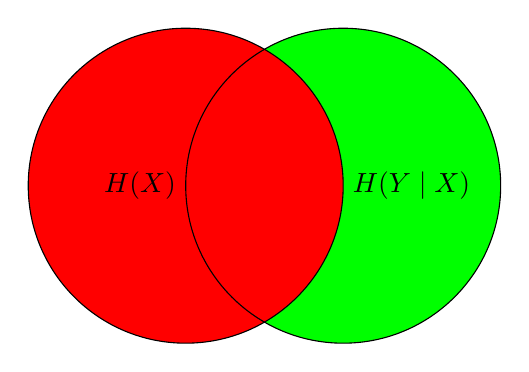
\begin{tikzpicture}
    \def\HX{(0,0) circle (2)}
    \def\HY{(2,0) circle (2)}
    \def\HYX{(1,0)}
    \begin{scope}%[fill opacity=0.75]
      \fill[green] \HY;
      \fill[red] \HX;
      \draw \HX node[left] {$H(X)$};
      \draw \HY node[right] {$H(Y\mid X)$};
    \end{scope}
  \end{tikzpicture}
  \end{center}
\end{frame}

%\begin{frame}
%  \begin{proof}
%  \end{proof}
%\end{frame}

\begin{frame}
  \begin{corollary}
    \(H(\stoch X\mid \stoch Y) \leq H(\stoch X)\).
  \end{corollary}

  \begin{corollary}
    \(H(\stoch X\mid \stoch Y) = H(\stoch X)\) iff \(\stoch X\) and \(\stoch 
      Y\) independent.
  \end{corollary}
\end{frame}
%
%\begin{frame}
%  \begin{proof}
%  \end{proof}
%\end{frame}
%
%\begin{frame}
%  \begin{theorem}
%    Entropin för en Markovprocess
%  \end{theorem}
%\end{frame}

\subsection{Information density and redundancy}

\begin{frame}
  \begin{definition}
    \begin{itemize}
      \item Natural language \(L\).
      \item Stochastic variable \(\stoch P^n_L\) of strings of length \(n\).
      \item (Alphabet \(P_L\).)
      \item Entropy of \(L\) defined as
        \begin{align*}
          H_L = \lim_{n\to \infty}\frac{H(\stoch P^n_L)}{n}.
        \end{align*}
      \item Redundancy in \(L\) is
        \begin{align*}
          R_L = 1 - \frac{H_L}{\log |P_L|}.
        \end{align*}
    \end{itemize}
  \end{definition}
\end{frame}

\begin{frame}
  \begin{remark}
    Meaning we have \(H_L\) bits per character in \(L\).
  \end{remark}

  \begin{example}[\cite{Shannon1948amt}]
    \begin{itemize}
      \item Entropy of 1--1.5 bits per character in English.
      \item Redundancy of approximately \(1 - \frac{1.25}{\log 26} \approx 
          0.73\).
    \end{itemize}
  \end{example}

\end{frame}

\begin{frame}
  \begin{example}[\cite{Shannon1948amt}]
    Two-dimensional cross-word puzzles requires redundancy of approximately 
    \(0.5\).
  \end{example}

  \begin{example}
    \begin{itemize}
      \item Redundancy of \enquote{SMS languages} is lower than for 
        \enquote{non-SMS languages}.

      \item Compare \enquote{också} and \enquote{oxå}.

    \end{itemize}
  \end{example}

  \begin{remark}
    \begin{itemize}
      \item Lower redundancy is more space-efficient.
      \item Incurs more errors.
    \end{itemize}
  \end{remark}
\end{frame}

%\begin{frame}
%  \begin{itemize}
%    \item Detta säger också att vi kan uppskatta entropin för en given 
%      Markovprocess.
%
%    \item Shannon modellerade språket som en Markovprocess i sin artikel 
%      \cite{Shannon1948amt}.
%
%    \item Vi kan även beräkna entropin för ett givet tillstånd i en 
%      Markovprocess genom betingad entropi.
%
%  \end{itemize}
%\end{frame}

\subsection{Information gain}

\begin{frame}
  \begin{definition}
    \begin{itemize}
      \item Set \(U\) of possible outcomes.
      \item Probability of outcome \(u\in U\) denoted \(p_u\).
      \item We learn that some \emph{unknown} outcome is in \(A\subset U\).
      \item Then the \emph{information gain} \(G(A\mid U)\) is defined as
        \begin{align*}
          G(A\mid U) = \log\frac{1}{\Pr(A)} = -\log\Pr(A),
        \end{align*}
        where \(\Pr(A) = \sum_{i\in A} p_i\).
    \end{itemize}
  \end{definition}
\end{frame}

\begin{frame}
  \begin{example}[Roll of dice again]
    \begin{itemize}
      \item Someone rolls and we should guess the result, \(\frac{1}{6}\) 
        chance.
      \item We learn that it was an even number, we gain
        \begin{align*}
          -\log\left( \frac{1}{6} + \frac{1}{6} + \frac{1}{6}\right) =
          -\log\frac{3}{6} = \log\frac{6}{3} = \log 2 = 1.
        \end{align*}
      \item The remaining uncertainty is \SI{1.58}{\bit}.
    \end{itemize}
  \end{example}

  \pause{}

  \begin{remark}
    \begin{itemize}
      \item \(X' = \{\fcdice{2}, \fcdice{4}, \fcdice{6}\}\)
      \item \(H(\stoch X') = - \sum_{x\in X'} \Pr(\stoch X' = x)\log \Pr(\stoch 
          X' = x)\)
      \item I.e.\ \(- 3 \times \frac{1}{3}\log\frac{1}{3} \approx 1.58\).
    \end{itemize}
  \end{remark}
\end{frame}

\begin{frame}
  \begin{example}[Dice yet again]
    \begin{itemize}
      \item We learn the die show less than five, i.e.\ not \fcdice{5} nor 
        \fcdice{6}.
      \item This yields
        \begin{align*}
          -\log\left( 4\times\frac{1}{6}\right) = \log\frac{6}{4}\approx 0.58
        \end{align*}
    \end{itemize}
  \end{example}
\end{frame}


\section[Applications]{Application in security}

\subsection{Passwords}

\begin{frame}
  \begin{block}{Idea~\cite{Komanduri2011opa}}
    \begin{itemize}
      \item Look at different aspects of passwords individually, then 
        summarize.
      \item Can use \(H(x_1, x_2, \ldots, x_n) \leq H(x_1) + H(x_2) + \cdots 
          + H(x_n)\).
      \item This allows us to reason about bounds.
    \end{itemize}
  \end{block}
\end{frame}

\begin{frame}
  \begin{example}
    \begin{itemize}
      \item We can look at properties such as:
        \begin{itemize}
          \item length,
          \item number of and placement of character classes,
          \item the actual characters,
          \item \dots
        \end{itemize}
    \end{itemize}
  \end{example}

  \pause{}

  \begin{remark}
    \begin{itemize}
      \item These are \emph{not independent}.
      \item The sum will be an \emph{upper bound}.
    \end{itemize}
  \end{remark}
\end{frame}

\begin{frame}
  \begin{remark}
    \begin{itemize}
      \item With an upper bound we know it's not possible to do better.
      \item With an average we know how well most users will do.
      \item With a lower bound we have a guarantee --- not possible!
    \end{itemize}
  \end{remark}
\end{frame}

\begin{frame}
  \begin{remark}
    \begin{itemize}
      \item If a password policy yields low entropy, it implies it's bad.
      \item If a password policy yields high entropy, it \emph{doesn't} imply 
        that it's good.
    \end{itemize}
  \end{remark}

  \pause

  \begin{exercise}
    Why?
  \end{exercise}
\end{frame}

\begin{frame}
  \begin{figure}
    \includegraphics[height=0.7\textheight]{password_strength.png}
    \caption{xkcd's strip on password strength.
    Picture: xkcd~\cite{xkcd936}.}
  \end{figure}
\end{frame}

%\begin{frame}{En förklaring av xkcd}
%  \begin{itemize}
%    \item Vi har 1 miljon engelska ord: ger \(\log 10^6 \approx 20\) bitar 
%      entropi.
%      (xkcd använder 16 bitar, vilket ger ca 70\,000 ord, alla ord i engelskan 
%      är inte vanliga.)
%
%    \item Vi kan ha inledande versal: ger 1 bit entropi.
%
%    \item Vi har några vanliga substitutioner: uppskattningsvis 10 stycken, 
%      d.v.s.~3 bitar entropi.
%
%    \item Vi har specialtecken (ej substitution): uppskattningsvis 4 bitar 
%      entropi.
%
%    \item Vi har siffror: \(\log 10\approx 3\).
%
%    \item Ordningen på specialtecknet och siffran: ger 1 bit entropi.
%
%    \item Totalt 32 bitar entropi:
%      \begin{itemize}
%        \item Tar minst 50 dagar med 1\,000 gissningar per sekund.
%        \item Tar strax över en timme med 1\,000\,000 gissningar per sekund.
%      \end{itemize}
%
%  \end{itemize}
%\end{frame}

\begin{frame}
  \begin{example}[Standard password]
    \begin{itemize}
      \item We have
        \begin{itemize}
          \item 26 alphabetic characters,
          \item 10 numbers,
          \item 10 special characters (approximately).
        \end{itemize}

      \item This yields \(\log( 2\times 26 + 10 + 10 ) = \log 72 \approx 
          \SI{6}{\bit}\) per password character.

      \item A 10-character \emph{uniformly randomly} generated password 
        contains \SI{60}{\bit}.
    \end{itemize}
  \end{example}

  \pause{}

  \begin{remark}
    What happens when we require two upper and two lower-case characters, two 
    numbers must be included?
  \end{remark}
\end{frame}

\begin{frame}
  \begin{example}[Four-word passphrase]
    \begin{itemize}
      \item We have 125\,000 words in the standard Swedish dictionary.
      \item This yields \(\log 125\,000\approx \SI{17}{\bit}\) per word.
      \item A four-word \emph{uniformly randomly} generated passphrase contains
        \SI{68}{\bit}.
    \end{itemize}
  \end{example}
\end{frame}

\begin{frame}
  \begin{example}[Random sentence]
    \begin{itemize}
      \item We estimated the entropy per character in a language.
      \item It was approximately \(\SI{1.25}{\bit}\) for English.
      \item A 20-character \emph{uniformly randomly} generated sentence would 
        yield \SI{25}{\bit}.
    \end{itemize}
  \end{example}
\end{frame}

\begin{frame}
  \begin{remark}
    \begin{itemize}
      \item All these require uniform randomness.
      \item Humans are bad at remembering random things.
      \item Thus they will choose non-randomly.
      \item The entropy will thus be (possibly much) lower.
    \end{itemize}
  \end{remark}
\end{frame}

\subsection{Research about human chosen passwords}

\begin{frame}
  \begin{example}[\citetitle{Bonneau2012lpo}~\cite{Bonneau2012lpo}]
    \begin{itemize}
      \item Investigates how linguistics affect the choice of multi-word 
        passphrases.

      \item Users don't choose them randomly, prefer adapted to natural 
        language.

      \item \enquote{correct horse battery staple} is preferred to 
        \enquote{horse correct battery staple} since the first is more 
        grammatically correct.
    \end{itemize}
  \end{example}
\end{frame}

\begin{frame}
  \begin{example}[\citetitle{Kuo2006hso}~\cite{Kuo2006hso}]
    \begin{itemize}
      \item Studied how users creates easy-to-remember passwords.

      \item Also investigated the strength of phrase-based passwords.

      \item E.g.\ Google's example \enquote{To be or not to be, that is the 
          question}\footnote{%
          URL\@: 
          \protect\url{http://www.lightbluetouchpaper.org/2011/11/08/want-to-create-a-really-strong-password-dont-ask-google/}.
        } which results in \enquote{2bon2btitq}.

      \item This particular password has apparently been used by many \dots
    \end{itemize}
  \end{example}
\end{frame}

\begin{frame}
  \begin{remark}
    \begin{itemize}
      \item There is a PhD thesis on the topic of guessing passwords: 
        \fullcite{GuessingHumanChosenSecrets}.
      \item There is even a conference dedicated to passwords: PasswordsCon.
    \end{itemize}
  \end{remark}
\end{frame}

\subsection{Identifying information}

\begin{frame}
  \begin{example}
    Do we get more information from zodiac signs or birthdays?
    \begin{align*}
      -\sum_{\mathclap{\text{zodiacs}}} \frac{1}{12} \log\frac{1}{12} &= \log 12 
      \approx 3.58 \\
      &< -\sum_{\mathclap{\text{days of year}}} \frac{1}{365} \log\frac{1}{365} 
      = \log 365 \approx 8.51.
    \end{align*}
  \end{example}
\end{frame}

\begin{frame}
  \begin{exercise}
    How much information do we need to uniquely identify an individual?
  \end{exercise}
\end{frame}

\begin{frame}
  \begin{example}
    \begin{itemize}
      \item Sometime during 2011 there were \(n = 6\,973\,738\,433\)\footnote{%
          According to the World Bank.
        } people on earth.

      \item To give everyone a unique identifier we need \(\log n\approx 
          32.7\approx 33\) bits of information.
    \end{itemize}
  \end{example}
\end{frame}

\begin{frame}
  \begin{block}{Identifying information in browsers}
    \begin{itemize}
      \item Electronic Frontier Foundation (EFF) studied~\cite{Eckersley2010hui} 
        how much information a web-browser shares.

      \item You can try your browser in \url{http://panopticlick.eff.org/}.
    \end{itemize}
  \end{block}

  \pause{}

  \begin{example}[My browser]
    \begin{itemize}
      \item My Firefox-browser with all addons gave 21.45 bits of entropy.

      \item Then the number of tested users were 2\,860\,696.
    \end{itemize}
  \end{example}
\end{frame}

\begin{frame}
  \begin{figure}
    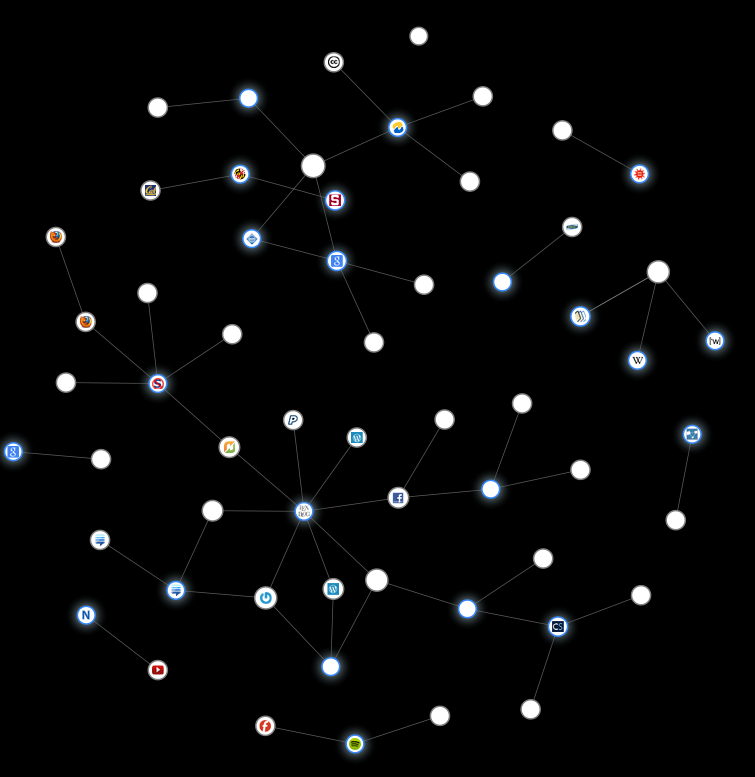
\includegraphics[height=0.7\textheight]{collusion.png}
    \caption{Screenshot from Collusion (now Lightbeam) for Firefox.
      Map over all pages that track me using this information.}
  \end{figure}
\end{frame}


%%%%%%%%%%%%%%%%%%%%%%

\subsection*{References}
\begin{frame}[allowframebreaks]
	\small
  \printbibliography{}
\end{frame}

\end{document}
